% !TEX TS-program = XeLaTeX
% !TEX encoding = UTF-8 Unicode

\chapter{实现与测试}
\label{chap07}
\defaultfont

\section{系统环境}

\subsection{硬件环境}

\begin{enumerate}
  \item CPU:Intel(R) Core(TM) i7-7700HQ CPU @ 2.80GHz   2.80 GHz
  \item 内存:16.0 GB
  \item 硬盘容量:500GB
\end{enumerate}

\subsection{软件环境}

\begin{enumerate}
  \item 操作系统:Windows 10 家庭中文版(20H2)作为编辑环境+ WSL2(Ubuntu 20.04)作为开发环境
  \item 数据库:mysql Ver 8.0.23-0ubuntu0.20.04.1 for Linux on x86\_64 (Ubuntu)
  \item 客户端:主流浏览器
\end{enumerate}


\section{持久化}
\subsection{Spring Date \& JPA Hibernate}

\begin{enumerate}
  \item 使用“逻辑模型工具”(例如Navicat Data Module 3)建立模型。
  \item 将模型同步至数据库
  \item 使用IDEA持久化工具生成实体类
  \item 根据逻辑模型为实体类添加注解(实现级联关系)
\end{enumerate}

关键问题如下:

\begin{enumerate}
  \item 多对一,一对多关系实现\\
        这种关系一共有四种实现方式
        \begin{enumerate}
          \item 单向\lstinline[language = Java]| @OneToMany |绑定
          \item 带有\lstinline[language = Java]| @JoinColumn |的单向\lstinline[language = Java]| @OneToMany |绑定
          \item 双向\lstinline[language = Java]| @OneToMany , @ManyToOne|绑定
          \item 不带有\lstinline[language = Java]| ManyToOne |的双向绑定
        \end{enumerate}
        本系统采用第三种方式
        \begin{lstlisting} [language = Java]
    public class A { //  一方
        ...
        @OneToMany(...)
        private List<B> bs;
        ...
    }
    public class B { // 多方
        @ManyToOne
        @JoinColumn(name = "a_id", referencedColumnName = "id")
        private A a;
    }
\end{lstlisting}
  \item 级联更新
        \begin{enumerate}
          \item 在“一方”(A)中 \lstinline[language = Java]| @OneToMany(cascade = CascadeType.ALL) |
          \item "深拷贝"A中的 \lstinline[language = Java]| BCopy = List<B> |
          \item 清空A中的 \lstinline[language = Java]| List<B> |
          \item \lstinline[language = Java]| BRepository.deleteAll(BCopy) |
          \item \lstinline[language = Java]| ARepository.save(A) |
        \end{enumerate}
  \item 级联查询
        \begin{enumerate}
          \item Dao层:继承JpaSpecificationExecutor
                \begin{lstlisting} [language = Java]
    public interface ARepository extends 
        JpaRepository<A, Integer>, 
        JpaSpecificationExecutor<AEntity> // 注意这里
\end{lstlisting}
          \item Service层使用:
                \begin{lstlisting} [language = Java]
    aRepository.findAll(new Specification<A>() {
        @Override
        // Hibernate根据此方法生成过滤语句
        public Predicate toPredicate(
            Root<UnfinishedPlanEntity> root, 
            CriteriaQuery<?> query, 
            CriteriaBuilder criteriaBuilder) {
          // 实现逻辑
        }
    })             
\end{lstlisting}
                涉及的重要的类:
                \begin{enumerate}
                  \item \lstinline[language = Java]| javax.persistence.criteria.Path |:通过实体类属性名获取字段值
                  \item \lstinline[language = Java]| javax.persistence.criteria.Join |:通过实体类属性名级联
                  \item \lstinline[language = Java]| javax.persistence.criteria.CriteriaBuilder |:拼接生成过滤
                \end{enumerate}
        \end{enumerate}
\end{enumerate}

\section{登陆\&验证授权模块}

\subsection{JWT优势}

随着Web应用规模的逐渐扩大,传统的基于Session和cookie的身份验证技术逐渐显现出它的弊端。
随着服务器的不断增加,由于多个请求可以被分发给不同的服务器,那么此时,服务器该如何那些请求来自同一个用户,对此有两种解决方式
\begin{enumerate}
  \item 多个服务器之间同步用户状态,这样无论用户的请求分发到哪一个服务器,都可以操作用户状态
  \item 判断来自同一个用户的请求,将同一个用户的请求一直分发到同一个服务器
\end{enumerate}
很显然,无论是上述哪种方式,随着用户量的增长开销都会变得很大。
例如第一种方式可以使用会话复制实现,Sesson复制性能也会随着服务器的增加而急剧下降。\cite{.2019h}

JWT(JSON Web Token)的优势在于
\begin{enumerate}
  \item 将用户认证信息保存在客户端,减轻服务器的存储压力。
  \item 提供无状态的身份认证——不需要服务器端多端同步用户状态,利于分布式应用开发。\cite{.2019h}
\end{enumerate}


\subsection{使用JWT\&Spring Security 实现验证和授权}

\begin{figure}[ht]
  \centering
  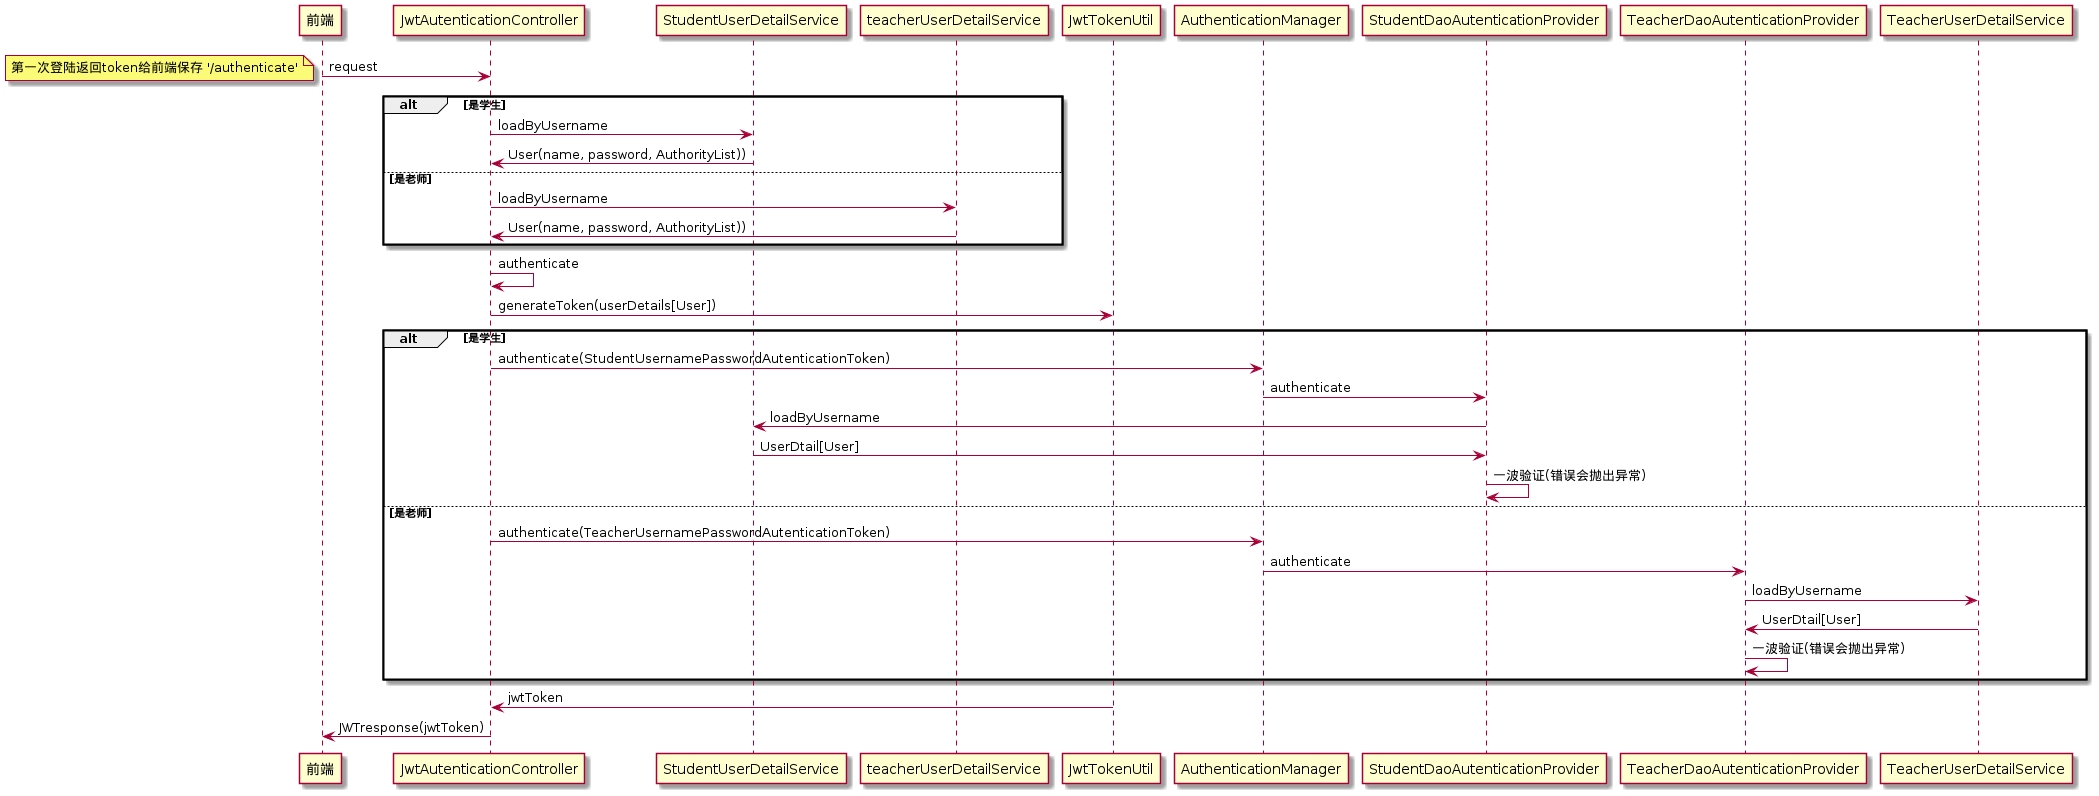
\includegraphics[scale = 0.3, angle = 90]{out/uml/时序图/时序图-authentication/时序图-authentication.png}
  \caption{\song\wuhao 登陆验证授权时序图}
\end{figure}

关键问题如下:
\begin{enumerate}
  \item 后端配置多用户表使用Spring Security\\
        验证授权涉及到的关键类(图\ref{SpringSecurity}):
        \begin{figure}[ht]
          \centering
          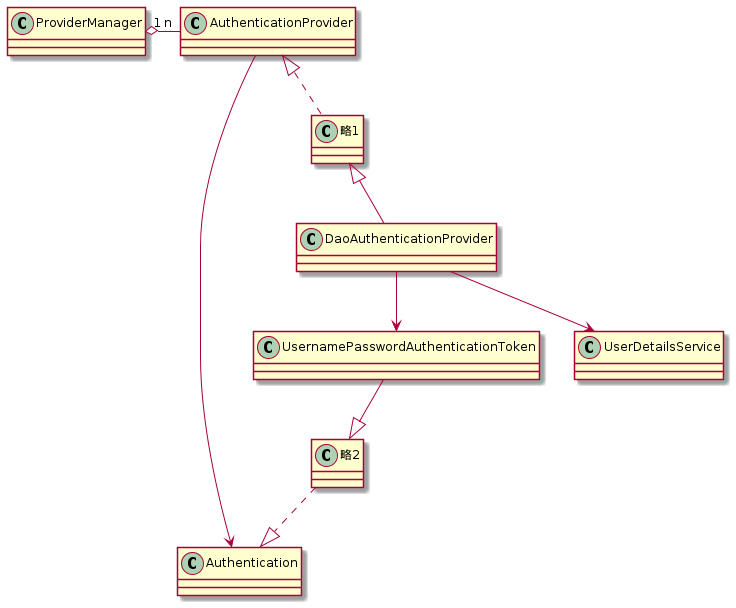
\includegraphics[scale = 0.5]{out/uml/类图/Spring Security/SpringSecurity验证/SpringSecurity验证.png}
          \caption{\song\wuhao Spring Security 验证授权关键类}
          \label{SpringSecurity}
        \end{figure}
        \begin{enumerate}
          \item \lstinline[language = Java]| Authentication |:用户认证信息。
          \item \lstinline[language = Java]| UsernamePasswordAuthenticationToken |:\lstinline[language = Java]| Authentication |的实现类,用于登陆验证,最为常用。
          \item \lstinline[language = Java]| AuthenticationProvider |:认证器,不同的\lstinline[language = Java]| AuthenticationProvider | 处理不同的 \lstinline[language = Java]| Authentication |
          \item \lstinline[language = Java]| DaoAuthenticationProvider |:\lstinline[language = Java]| AuthenticationProvider |的实现类,用于处理\lstinline[language = Java]| UsernamePasswordAuthenticationToken |
          \item \lstinline[language = Java]| ProviderManager |:用于管理\lstinline[language = Java]| AuthenticationProvider |
          \item \lstinline[language = Java]| UserDetailService |:为\lstinline[language = Java]| DaoAuthenticationProvider |提供从数据库查询用户的功能,用于做密码对比。
        \end{enumerate}
        多用户表配置Spring Security(图\ref{SpringSecurityMultiUser}):
        \begin{enumerate}
          \item 为不同用户建立各自的\lstinline[language = Java]| UserDetailService |
                \begin{lstlisting} [language = Java]
    public class XXXUserDetialsService 
                implements UserDetailService
                \end{lstlisting}
                ,各自的\lstinline[language = Java]| UserDetailService |从各自的数据库表中查询密码,提供给各自的\lstinline[language = Java]| DaoAuthenticationProvider |使用。
          \item 为不同用户建立各自的\lstinline[language = Java]| UsernamePasswordAuthenticationToken | \begin{lstlisting} [language = Java]
    public class XXXUPAuthToken 
                extends UsernamePasswordAuthenticationToken
              \end{lstlisting}
          \item 为不同用户建立各自的\lstinline[language = Java]| DaoAuthenticationProvider | \begin{lstlisting} [language = Java]
    public class XXXDaoAuthProvider 
                extends DaoAuthenticationProvider
              \end{lstlisting}
          \item 进行Security配置 \begin{lstlisting} [language = Java]
    @Configuration
    @EnableWebSecurity
    @EnableGlobalMethodSecurity(prePostEnabled = true)
    public class MySecurityConfig 
                extends WebSecurityConfigurerAdapter 
              \end{lstlisting}
                需要的关键配置:\begin{enumerate}
                  \item 注入\lstinline[language = Java]| XXXAuthProvider |
                  \item 向\lstinline[language = Java]| AuthenticationManager |添加\lstinline[language = Java]| XXXAuthProvider |
                  \item 注入\lstinline[language = Java]| AuthenticationManager |
                \end{enumerate}
        \end{enumerate}
        总体流程:
        \begin{enumerate}
          \item 前端发起身份验证请求,由于尚未登陆,所以前端没有Token信息,因而无法通过Spring Security的验证,这需要在 MySecurityConfig 中配置——放过访问"/authentication"的请求,以便进行身份验证和授权。\begin{lstlisting} [language = Java]
  @Override
  protected void configure(HttpSecurity httpSecurity)
                                    throws Exception {
    httpSecurity.authorizeRequests()
        .antMatchers("/authenticate", "/register")
        .permitAll()// 身份验证和注册不需要拦截
        ...
  }
              \end{lstlisting}
          \item 请求到达 MyAuthenticationController,此时可以从请求中获取到登陆用户身份类型,如果是学生则需要使用 StudentUserDetailService 获取UserDetails,如果是教师则需要使用 TeacherDetailsService 获取UserDetails,同理,如果是管理员则需要使用 AdminDetailsService 获取UserDetials。
          \item 此时进入到 XXXUserDetialsService 中,这里需要重写方法 loadUserByUsername(String username),如果是为学生用户服务的,则需要根据传入的username从学生表中取出用户,如果是为教师服务的,则需要查询教师表并从中找到用户。如果没有找到用户则抛出异常,如果找的了则建立 org.springframework.security.core.userdetails.User(为UserDetials的实现类)其中包含用户名,用户密码,用户权限和用户身份。
          \item 当获得了 XXXUserDetialsService 返还的 UserDetials,则可以开始进行身份验证。该验证需要 AuthenticationProvider 来完成,因此需要传递需要验证的东西(Authentication)给管理 AuthenticationProvider 的 AuthenticationManager 进行身份验证。由于这里有不同种类的用户且不同种类用户需要查询不同的表,所以需要建立不同 AuthenticationProvider (使用不同的 XXXUserDetialsService(从不同的数据库查询用户))去处理不同的 Authentication,而用来处理用户名用户密码的 AuthenticationProvider 是 DaoAuthenticationProvider,用来处理用户名用户密码的 Authentication 是 UsernamePasswordAuthenticationToken,所以需要为不同用户建立不同的 XXXUsernamePasswordAuthenticationToken 和不同的 XXXAuthProvider。为了绑定 XXXAuthProvider 和 XXXUsernamePasswordAuthenticationToken 则需要重写 XXXAuthProvider 的 supports 方法。
                \begin{lstlisting} [language = Java]
    // XXXDaoAuthProvider
    @Override
    public boolean supports(Class<?> authentication) {
        return XXXUsernamePasswordAutenticationToken
                .class
                .isAssignableFrom(authentication);
    }
              \end{lstlisting}
                DaoAuthenticationProvider 是继承 AbstractUserDetailsAuthenticationProvider 的,不同在于 DaoAuthenticationProvider 增加了验证密码的功能,这也正是我们需要的,但是验证密码需要查询数据库也就需要 UserDetailService,所以需要通过 MySecurityConfig 为 XXXAuthProvider 注入不同的 XXXUserDetialsService。这里选择setter注入:
                \begin{lstlisting} [language = Java]
  // XXXDaoAuthProvider
  @Override
  public void setUserDetailsService(
      UserDetailsService userDetailsService) {
      super.setUserDetailsService(userDetailsService);
  }
              \end{lstlisting}
                \begin{lstlisting} [language = Java]
  // MySecurityConfig
  @Autowired
  @Qualifier("XXXUserDetailsService")
  private UserDetailsService XXXUserDetailsService;

  // 注入
  @Bean("XXXDaoAutenticationProvider")
  DaoAuthenticationProvider daoXXXDaoAutenticationProvider() 
  {
    return new XXXDaoAutenticationProvider(
                                passwordEncoder(), 
                                XXXUserDetailsService);
  }
              \end{lstlisting}
                这个过程中涉及的类比较多且关系比较笔复杂,可以参考图\ref{SpringSecurityMultiUser}(经过简化,略去了与该流程相关程度不大的类)。
          \item 之后流程又回到了 MyAuthenticationController,此时如果通过了之前的身份验证则可以为用户生成Token了,这里需要使用 JwTokenUtil 生成Token,将 之前获得的 userdetails 传递给 JwTokenUtil,需要注意的是要在 claims 中填入用户角色,这样前端拿到Token之后可以解析出用户角色(这部分信息对应图\ref{jwt}Payload部分)。
                \begin{lstlisting} [language = Java]
  // 后端生成Token
  public String generateToken(UserDetails userDetails) {
      Map<String, Object> claims = new HashMap<>();
      Collection<? extends GrantedAuthority> it = 
                          userDetails.getAuthorities();

      List<String> roles = new ArrayList<String>();
      for (GrantedAuthority grantedAuthority : it) {
          System.out.println(grantedAuthority.toString());
          if (grantedAuthority.toString()
                          .startsWith("ROLE_")) {
              roles.add(
                  grantedAuthority.toString().substring(5));
          }
      }
      
      claims.put("userType", roles); 
          // 在 JWT payload 中放入 自定义的角色信息

      return doGenerateToken(
              claims, userDetails.getUsername());
  }
              \end{lstlisting}
                \begin{lstlisting} [language = Java]
  // 前端解析Token
  export function jwtDecrypt(token) {
    var base64Url = token.split('.')[1];
    var base64 = base64Url.replace(/-/g, '+')
                            .replace(/_/g, '/');
    var jsonPayload = decodeURIComponent(
      atob(base64)
      .split('')
        .map(function (c) {
          return '%' + ('00' + 
            c.charCodeAt(0).toString(16)).slice(-2);
        })
        .join('')
    );
    return JSON.parse(jsonPayload);
  }
                \end{lstlisting}
          \item 当前端接收到后端的response之后,则可以从返还的Token中获取用户信息存储到localStore。之后的每个请求也都需要在Header中放入Token用于身份验证。
        \end{enumerate}
        \begin{figure}[ht]
          \centering
          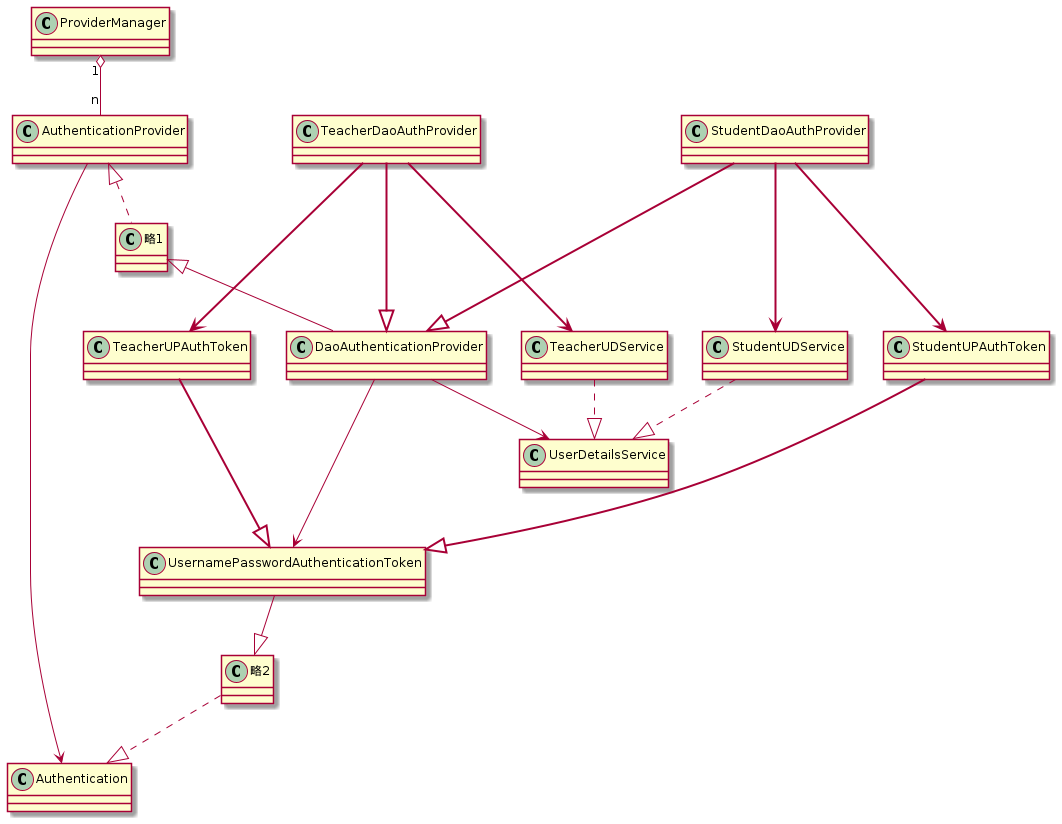
\includegraphics[scale = 0.35]{out/uml/类图/Spring Security/SpringSecurity多用户表验证/SpringSecurity多用户表验证.png}
          \caption{\song\wuhao SpringSecurity多用户表验证}
          \label{SpringSecurityMultiUser}
        \end{figure}
  \item 后端处理CORS跨域问题\\
        CORS(Cross-origin resource sharing)——跨域资源共享,一种可以允许访问其他域名下的受限资源的机制。
        目前CORS的现行标准由WHATWG(Web Hypertext Application Technology Working Group)在网络浏览器中实现和测试。\\
        CORS-preflight request——预检请求,对于可能会对服务器造成副作用的请求(非简单请求),浏览器会先使用OPTIONS方法发送预检请求
        询问服务器是否允许此次跨域请求。\\
        简单请求需满足:
        \begin{enumerate}
          \item 请求方法:\lstinline[language = xml]| GET、POST、HEAD |
          \item 只使用了如下的安全首部字段,不得人为设置其他首部字段\begin{lstlisting} [language = Java]
    Accept
    Accept-Language
    Content-Language
    Content-Type 仅限以下三种
            text/plain
            multipart/form-data
            application/x-www-form-urlencoded
    HTML头部header field字段:
                DPR、Download、Save-Data、Viewport-Width、WIdth
              \end{lstlisting}
          \item 请求中的任意XMLHttpRequestUpload 对象均没有注册任何事件监听器;XMLHttpRequestUpload 对象可以使用 XMLHttpRequest.upload 属性访问
          \item 请求中没有使用 ReadableStream 对象
        \end{enumerate}
        总的来说,在CORS问题中涉及两种请求:
        \begin{enumerate}
          \item CORS请求:CORS请求是一个包含“Origin”报头的HTTP请求。它不能被可靠地识别为参与了CORS协议,因为所有的方法既不是' GET '也不是' HEAD '的请求都包含了' Origin '头。
          \item CORS preflight请求:也就是所谓的预检请求,是检查CORS协议是否被理解的CORS请求。它使用' OPTIONS '作为方法,包括以下 header:
                \begin{enumerate}
                  \item \lstinline[language = Java]| Access-Control-Request-Method |:指示将来对同一资源的CORS请求可能使用的方法。
                  \item \lstinline[language = Java]| Access-Control-Request-Headers |:指示将来对同一资源的CORS请求可能使用的头。
                \end{enumerate}
                OPTIONS方法:用于描述对于目标资源的通信选项。客户端可以放松HTTP OPTIONS 请求来询问 web 服务器支持的 HTTP 方法和其他的选项。如果请求 URL 是一个 '*',那么 HTTP OPTIONS 请求应用于一般的服务器而不是特定的资源。使用HTTP OPTIONS方法的请求应该只检索数据(服务器不能更改其状态)。如果需要更改服务器上的数据,需要使用POST、PUT、PATCH或DELETE方法。
        \end{enumerate}
        在CORS问题中涉及的响应:
        \begin{enumerate}
          \item 对于CORS请求的响应可以包含下面的header:
                \begin{enumerate}
                  \item \lstinline[language = Java]| Access-Control-Allow-Origin |:通过在相应的header中添加被允许的Origin(可以为null也可以为'*')可以指示那些响应是否可以被分享。
                  \item \lstinline[language = Java]| Access-Control-Allow-Credentials |:指示当请求的凭据模式为"include"时响应是否可以被分享。
                  \item \lstinline[language = Java]| Access-Control-Expose-Headers |:通过列出header的名称来指示哪些header可以作为响应的一部分公开。
                \end{enumerate}
          \item 对于CORS preflight请求可以包含下面的header:
                \begin{enumerate}
                  \item \lstinline[language = Java]| Access-Control-Allow-Methods |:指示当请求目的为CORS协议时响应的URL支持那些请求方法。
                  \item \lstinline[language = Java]| Access-Control-Allow-Headers |:指示当请求的目的为CORS协议时相应的饿URL支持那些header。
                  \item \lstinline[language = Java]| Access-Control-Max-Age |:表示' Access-Control-Allow-Methods '和' Access-Control-Allow-Headers '头提供的信息可以被缓存的秒数(默认为5)
                \end{enumerate}
        \end{enumerate}
        CORS流程(图\ref{CORS-flow}):
        \begin{figure}[ht]
          \centering
          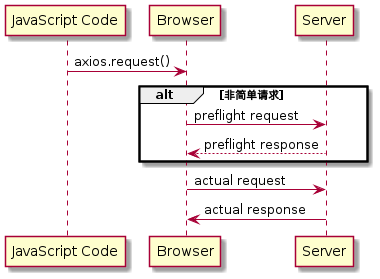
\includegraphics[scale = 0.6]{out/uml/时序图/CORS-flow/CORS-flow.png}
          \caption{\song\wuhao CORS流程}
          \label{CORS-flow}
        \end{figure}
        Spring Security 配置配置CORS:
        \begin{enumerate}
          \item 打开CORS \begin{lstlisting} [language = Java]
// MySecurityConfig.java
  protected void configure(HttpSecurity httpSecurity) 
                            throws Exception {
    httpSecurity..cors()
              \end{lstlisting}
          \item 配置配置CORS response
                \begin{lstlisting} [language = Java]
// MySecurityConfig.java
@Bean
CorsConfigurationSource corsConfigurationSource() {
  CorsConfiguration configuration = new CorsConfiguration();
  configuration.addAllowedOrigin("*"); 
                // 应设置为前端服务器域名前缀
  configuration.setAllowedMethods(
              Arrays.asList("GET", "POST", "OPTION"));
  configuration.addAllowedHeader("*");
  // 允许的Header,起码需要允许 Access-Control-Allow-Origin
  UrlBasedCorsConfigurationSource source = 
                          new UrlBasedCorsConfigurationSource();
  source.registerCorsConfiguration("/**", configuration);
  return source;
}
          \end{lstlisting}
        \end{enumerate}
  \item 前端对Token的处理\\
        这里使用Vuex进行管理,为身份验证单独创建一个 auth 模块。
        \begin{lstlisting} [language = Java]
// src/store/index.js
import {
  createStore
} from 'vuex'
import authModule from './modules/auth'

const store = createStore({
  modules: {
    auth: authModule,
  }
})

export default store;

    \end{lstlisting}
        \begin{enumerate}
          \item 在 auth.js 的 state 中: 创建一个 authDate 对象,其中保存用户的Token,refreshToken,tokenExp,userId,userName,userType,以及一个loginStatus。
          \item 在 auth.js 的 getter 中:创建 getLoginStatus() 用于获取用户的登陆状态(是否登陆),创建 getAuthDate() 用于获取用户的身份信息,创建 isTokenActive() 用于判断 Token 是否过期。
          \item 在 auth.js 的 mutations 中:创建 saveTokenDate() 用于更新 authDate 以及 将 token 保存在浏览器的 localStorage 中。创建 setLoginStatus() 用于更新登陆状态。创建 signout() 用于登出(清除localStorage中的Token,以及将登陆状态更改为未登陆)。
          \item 在 auth.js 的 actions 中:创建异步函数 login() 用于登陆(使用 axios 发送请求,将 paylaod(username, password, usertype) 放在请求体中发送给后端,使用 mutations 中方法处理返回的结果,成功登陆。
        \end{enumerate}
  \item 前端配置导航守卫\\
        本系统添加全局的前置守卫:使用 \lstinline[language = Java]| router.beforeEach |,该方法接收三个参数,to,from,next(其中第三个参数可选)
        \begin{enumerate}
          \item to:想要导航到的规范化格式的目标路由位置。
          \item from:其格式为规范化,表示导航时当前的即正要离开的路由位置。
          \item next:经过判断后应该导航到的路由位置。
        \end{enumerate}
        配置的导航守卫的大体思路是只要未登陆都需要跳转到 login 界面,但是如果访问 login 界面,此时系统尚未登陆,然后又会跳转到 login 界面,无限跳转,无法正常工作。所以这里为每个页面的路由设置一个参数 requiredAuth 用于指示该页面是否需要导航守卫。设置方法如下:
        \begin{lstlisting} [language = Java]
// src/router/index.js
import Login from '../components/Login.vue'
const routes = [
{
  path: '/login',
  name: 'Login',
  component: Login,
  meta: {
    requiredAuth: false
  }
},
]
    \end{lstlisting}
        导航守卫流程:
        \begin{enumerate}
          \item 检查 store 中是否保存了 token,如果没有保存则需要从 localStorage 中获取并保存在 store 中。
          \item 调用 auth 模块 中的 isTokenActive getter,从而获知该 Token 是否过期。
          \item 如果 Token 尚未过期并且想要导航到的目标路由需要验证\\meta.requiredAuth === true)则跳转到系统首页,如果并不满足上述条件则需要跳转到 login 页面。
        \end{enumerate}
  \item 为每个请求附带 Token\\
        思路为进行全局配置,在 axios 发送每个请求之前在 Header 中添加 authenticate 字段,其值为登陆时从后端获取的 Token。

        使用 axios 的 interceptors(拦截器)实现。interceptors 主要可以分成两种:
        \begin{enumerate}
          \item 处理 request
                \begin{lstlisting} [language = Java]
// 添加一个请求拦截器
axios.interceptors.request.use(function (config) {
    // 在请求发送前的一些处理
    return config;
  }, function (error) {
    // 在请求错误前的一些处理
    return Promise.reject(error);
  });

                \end{lstlisting}
          \item 处理 response
                \begin{lstlisting} [language = Java]
// 添加一个响应拦截器
axios.interceptors.response.use(function (response) {
    // 任何处于2xx范围内的状态代码都会触发此函数
    // 处理返回的数据
    return response;
  }, function (error) {
    // 任何超出2xx范围的状态码都会触发该函数
    // 处理响应错误
    return Promise.reject(error);
  });
\end{lstlisting}
        \end{enumerate}
        系统需要为请求添加拦截器:
        \begin{lstlisting} [language = Java]
// main.js
axios.interceptors.request.use((config) => {
  const authData = store.getters['auth/getAuthData'];
  config.headers.common.Authorization = 'bearer \${authData.token}';
  return config;
});
    \end{lstlisting}
        首先从 store 中获取用户身份信息,之后通过操作 config 对象在 header 中添加 Authorization 字段,值为用户身份信息当中保存的 token。在这样的里处理之后所有的请求都会在 header 中自动加入 token。
\end{enumerate}

\section{上传文件\&更新文件\&下载文件}

\subsection{上传文件}

\begin{enumerate}
  \item 前端配置\\
        前端使用 Elment Plus 的上传组件
        \begin{lstlisting} [language = Html]
<template>
  <div class="student_upload_paper_container0 container0">
    <el-upload
      class="upload-demo"
      action="http://localhost:8089/student/studentuploadpaper/"
      :on-success="handleSuccess"
      :on-preview="handlePreview"
      :on-remove="handleRemove"
      :before-remove="beforeRemove"
      multiple
      :on-exceed="handleExceed"
      :file-list="fileList"
      :data="{userName}"
      :auto-upload="true"
      list-type="text"
    >
      <button class="custom-btn btn-12 uploadButton">
        <span>Click!</span>
        <span>UPLOAD</span>
      </button>
      <template #tip>
        <div class="el-upload__tip"></div>
      </template>
    </el-upload>
  </div>
</template>
    \end{lstlisting}
        action:上传的地址,即后端定义的接口。

        multiple:设置可以多选文件。

        on-suscess:文件上传成功时的钩子。

        on-preivew:点击文件列表中已上传的文件时的钩子。

        on-remove:	文件列表移除文件时的钩子。

        auto-upload:是否在选取文件后立即进行上传。

        data:附带的数据,这里放入文件名字。

        file-list:文件列表数据。

  \item 后端配置
        \begin{enumerate}
          \item Controller:
                \begin{lstlisting} [language = Java]
    @PostMapping("/student/studentuploadpaper")
    public String studentUploadPaper(
        @RequestParam("file") MultipartFile file, 
        Principal principal) {
        \end{lstlisting}
                MultipartFile file:用来映射文件。

                Principal principal:从这里能取得发送请求的用户信息。
          \item Service:
                \begin{lstlisting} [language = Java]
    public StudentFileEntity store(
        MultipartFile file, String username) 
                                        throws IOException {
        String filename = StringUtils.cleanPath(
            file.getOriginalFilename());
        StudentFileEntity studentFileEntity = 
        new StudentFileEntity(filename, file.getContentType(), 
                            file.getBytes());

        studentFileEntity.setStudentByStudentId(
           studentRepository.findByName(username));
        return studentFileRepository.save(studentFileEntity);
    }
        \end{lstlisting}
                文件名字:从 file 中可以提取出文件名。

                拥有该文件的学生姓名:从 principal 中可以获取。

                文件数据:file.getBytes()

                文件类型:file.getContentType()

                至此,存储一个文件的所有信息已经获得,通过这些信息新建一个文件实体对象,使用文件Repository存储文件。
        \end{enumerate}
\end{enumerate}

\subsection{更新文件}

由于页面的结构,该功能并不适合使用 Elment Plus 的组件。

前端功能实现:
\begin{enumerate}
  \item 更新文件页面 template 部分:
        \begin{lstlisting} [language = Java]
 <input 
    type="file" 
    value="" 
    id="refreshFile" 
    @change="handleRefreshFile(\$event, file.id)">
 <label 
    for="refreshFile">
 </label>
    \end{lstlisting}
        需要一个选择文件的按钮。
  \item 更新文件页面 Script 部分:
        \begin{lstlisting} [language = Java]
  handleRefreshFile(e, id) {
    const file = e.target.files[0]
    const param = new FormData()
    param.append('file', file)
    param.append('id', id)
    param.append('name', file.name)
    const config = {
      headers: { 'Content-Type': 'multipart/form-data' }
    }
    this.studentRefreshFile({ param: param, config: config })
    .then((res) => {
      console.log('refresh file : ' + id);
    })
  },
    \end{lstlisting}
        \begin{enumerate}
          \item 获得文件 const file
          \item 新建 Form 表单
          \item 为表单填入文件,文件id,文件名
          \item 新建请求配置,配置 Content-Type 为 multipart/form-data
          \item 调用更新文件函数(传入参数文件和配置)
        \end{enumerate}
  \item 更新文件函数:
        \begin{lstlisting} [language = Java]
  async studentRefreshFile ({
    commit,
  }, payload) {
    const response = await axios.post(
      'http://localhost:8089/student/refreshFile', 
                            payload.param, payload.config)
    return response
  }
    \end{lstlisting}
\end{enumerate}
后端功能实现:
\begin{enumerate}
  \item Controller:
        \begin{lstlisting} [language = Java]
  public String refreshFile(@RequestParam("file") MultipartFile file
                              , @RequestParam("id") Integer id) {
  \end{lstlisting}
        使用 MultipartFile file 映射新上传的文件,使用 Integer id 映射需要被更新的文件的 id。
  \item Service:
        \begin{lstlisting} [language = Java]
  public void refreshFile(MultipartFile file, Integer id) 
                                                throws IOException {
      StudentFileEntity original_file = fileR.findById(id).get();
      original_file.setName(file.getOriginalFilename());
      original_file.setType(file.getContentType());
      original_file.setData(file.getBytes());
      fileR.save(original_file);
  }
  \end{lstlisting}
        首先从数据库取出原文件,更新文件的名称,文件的类型,文件的数据,之后重新保存回数据库。
\end{enumerate}

\subsection{下载文件}

\begin{enumerate}
  \item 前端请求函数:
        \begin{lstlisting} [language = Java]
  async studentDownloadThisFile({
    commit
  }, payload) {
    const response = await axios.get(
      'http://localhost:8089/student/downloadThisFile', {
      params: payload,
      responseType: 'arraybuffer'
    });
    return response;
  },
  \end{lstlisting}
        这里的重点是改变XMLHttpRequest对象的 responseType属性,将其设置为 "arraybuffer",否则返回的数据会被解析为 Json 对象,无法正确的处理文件,导致文件乱码。
  \item 后端处理函数:
        \begin{lstlisting} [language = Java]
  @GetMapping(value = "/student/downloadThisFile", 
                              produces = "application/pdf")
  public byte[] getMethodName(@RequestParam Integer fileId) {
      return fileService.downloadThisFile(fileId).getData();
  }
  \end{lstlisting}
        这里需要注意两点,
        
        第一点是一定要设置response的Content-Type为"application/pdf",设置方法为将produces参数赋值为"application/pdf"。
        
        第二点是因为本系统配置了统一返回对象,会对返回值在发送前进行封装,这次封装会导致返回的值不再是文件数据本身,所以需要设置不对 byte[] 类型进行重新封装。
        \begin{lstlisting} [language = Java]
@RestControllerAdvice
public class CustomResponseBodyAdvice implements 
                                      ResponseBodyAdvice<Object> {

    @Override
    public Object beforeBodyWrite(Object arg0, MethodParameter arg1, 
                                                    MediaType arg2,
            Class<? extends HttpMessageConverter<?>> arg3, 
            ServerHttpRequest arg4, ServerHttpResponse arg5) {
              ...
        } else if (arg0 instanceof byte[]) {
            return arg0;
        }
        ...
\end{lstlisting}
\end{enumerate}